\documentclass[12pt]{ctexart}
\usepackage{amsmath, amsthm, amssymb, bm, graphicx, hyperref, mathrsfs, enumitem, geometry, listings, fontspec, xcolor}
\title{杂谈勾股定理}
\author{无名氏}
\date{\today}
\newtheorem{theorem}{定理}[section]
\newtheorem{definition}[theorem]{定义}
\newtheorem{lemma}[theorem]{引理}
\newtheorem{corollary}[theorem]{推论}
\newtheorem{example}[theorem]{例}
\newtheorem{proposition}[theorem]{命题}
\begin{document}
\maketitle
\section{公式测试}

\newpage
\centering  
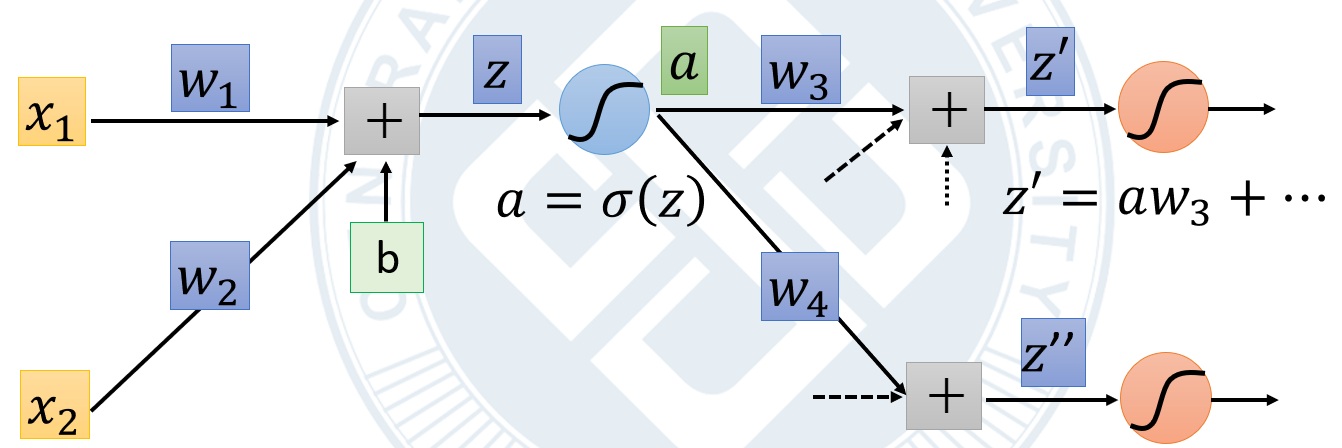
\includegraphics[width=\textwidth]{1.png} 
\label{fig:my_label}

已知:$z$为激活函数输入,$a$为激活函数输出和下一层的输入,$l$为损失函数。

$$z=w_1x_1+w_2x_2+b$$
$$a=\sigma (z)$$

每个权重参数的梯度计算方式为

\begin{equation}
    \begin{aligned}
        \frac{\partial l}{\partial w_1} &= \frac{\partial z}{\partial w_1} \cdot \frac{\partial l}{\partial z}\\
        &=\frac{\partial z}{\partial w_1} \cdot \frac{\partial a}{\partial z} \cdot \frac{\partial l}{\partial a}\\
        &=x_1 \cdot \frac{\partial a}{\partial z} \cdot \frac{\partial l}{\partial a}\\
        &=x_1 \cdot \sigma^\prime (z) \cdot \frac{\partial l}{\partial a}
    \end{aligned}
\end{equation}

发现只有$\frac{\partial l}{\partial a}$是未知的,需要继续计算。

\begin{equation}
    \begin{aligned}
        \frac{\partial l}{\partial a} &= \frac{\partial z^\prime}{\partial a} \cdot \frac{\partial l}{\partial z^\prime} 
        + \frac{\partial z^{\prime\prime}}{\partial a} \cdot \frac{\partial l}{\partial z^{\prime\prime}} 
        \\
        &= w_3 \cdot \frac{\partial l}{\partial z^\prime} + w_4 \cdot \frac{\partial l}{\partial z^{\prime\prime}}\\
        &= w_3 \cdot \sigma^\prime (z^\prime) \cdot \frac{\partial l}{\partial a^\prime} + w_4 \cdot \sigma^\prime (z^{\prime\prime}) \cdot  \frac{\partial l}{\partial a^{\prime\prime}}\\
        &= ...
    \end{aligned}
\end{equation}

\flushleft
发现从前向后计算梯度时,需要后续的所有的$\frac{\partial l}{\partial z}$或$\frac{\partial l}{\partial a}$的具体数值;而从后向前计算梯度,可以直接计算出梯度,并且计算结果可以在计算前层时直接使用,因此采用从后向前计算梯度的方式,即反向传播。


% $$ \frac{\partial l}{\partial w}= \frac{\partial w}{\partial z}\frac{\partial l}{\partial }$$
\end{document}